\setcounter{section}{1}
\section{Integration of Measurable Functions}

\begin{note}{Prop 2.3}
    Rigorously prove property (2). Let $h\in\mathcal{E}_+$ such that $h\le f$. Then if $h(x)>0, f(x)\ge h(x)>0$, so
    \[
    \{x\in E: h(x)>0\}\subset \{x\in E: f(x)>0\}
    \]
    Given $\mu(\{x\in E: f(x)>0\})=0$, so $\mu(\{x\in E: h(x)>0\})=0$. The integral of $h$ would be
    \[
    \int h\mathrm{d}\mu=\sum_{i=1}^n \alpha_i\mu(A_i)=0
    \]
    since either $\alpha_i=0$ or $\alpha_i>0$ but $\mu(A_i)=0$. Because $h\le f$ always holds,
    \[
    \int f\mathrm{d}\mu=\sup_{h\le f} \int h\mathrm{d}\mu=0
    \]
\end{note}

\begin{note}{Thm 2.4}
    \begin{enumerate}
        \item Why is $f$ measurable? 
        
        $f_n\to f\implies f=\limsup f_n=\liminf f_n$, then by Prop 1.14.
        \item Why $\int f \mathrm{d}\mu\ge \lim_n \int f_n \mathrm{d}\mu$? 
        
        Since $f_n$ is increasing, $f_n\le \lim_n f_n=f$. Take integrals, $\int f \mathrm{d}\mu\ge \int f_n \mathrm{d}\mu$, then take limit $n\to\infty$ on the RHS.
        \item Why $f_n\to f,a<1$ leads to $E_n\uparrow E$?

        We want to prove (1) $E_n\subset E_{n+1},\forall n$, (2) $\bigcup_{n=1}^{\infty}E_n=E$.

        (1) Take $x\in E_n, ah(x)\le f_n(x)\le f_{n+1}(x)$, so $x\in E_{n+1}$.

        (2) Let $x\in E,h(x)\le f(x),0\le a<1$. 
        \begin{enumerate}
            \item $h(x)=0$. Then $ah(x)=0\le f(x)$, so $x\in E_n,\forall n$.
            \item $h(x)>0$. Then $ah(x)<h(x)\le f(x)$. Since $f_n(x)\uparrow f(x), \exists N\in \mathbb{N}$, such that for $n\ge N,ah(x)<f_n(x)$. Thus $\forall n\ge N, x\in E_n$.
        \end{enumerate}
        We conclude that, $\forall x\in E,\exists N\in\mathbb{N}$, such that $\forall n\ge N,x\in E_n$, so
        \[\bigcup_{n\in\mathbb{N}}E_n=E\]
        Combined with $E_n\subset E_{n+1}, E_n\uparrow E$.
        \item Given $f_n\ge a\mathbf{1}_{E_n}h,$ then
        \[
        \int a\mathbf{1}_{E_n}h\mathrm{d}\mu=\int a\mathbf{1}_{E_n}\left(\sum_{i=1}^k \alpha_i \mathbf{1}_{A_i}\right)\mathrm{d}\mu=\int \left(a\sum_{i=1}^k \alpha_i \mathbf{1}_{E_n\cap A_i}\right)\mathrm{d}\mu=a\sum_{i=1}^k \alpha_i\mu(E_n\cap A_i)
        \]
        \item In the last step 
        \[
        \int h\mathrm{d}\mu\le \lim_{n\to\infty}\uparrow \int f_n \mathrm{d}\mu
        \]
        take $\sup_{h\in \mathcal{E}_+,h\le f}$ on both sides.
        \item Conclusion: 
        
        The most insightful part of this proof is to construct a simple function $h=\sum_{i=1}^k \alpha_i \mathbf{1}_{A_i}$ and restrict $h\le f$, then use Def 2.2.
    \end{enumerate}
\end{note}

\begin{note}{Prop 2.5}
    The author used constructive proof for (1). Recall uniform convergence: $\forall \varepsilon>0,\exists N\in\mathbb{N}$ such that $\forall n\ge N, x\in E, |f_n(x)-f(x)|<\varepsilon$. In uniform convergence, $N$ cannot depend on $x$. The constructed $f_n$ satisfies $0\le f-f_n\le 2^{-n}$ where $2^{-n}$ does not depend on $x$. 

    Example: $f(x)=2\sin(x)+2,n=3$, see Fig \ref{fig:prop2.5}.
    \begin{figure}[htbp]
        \centering
        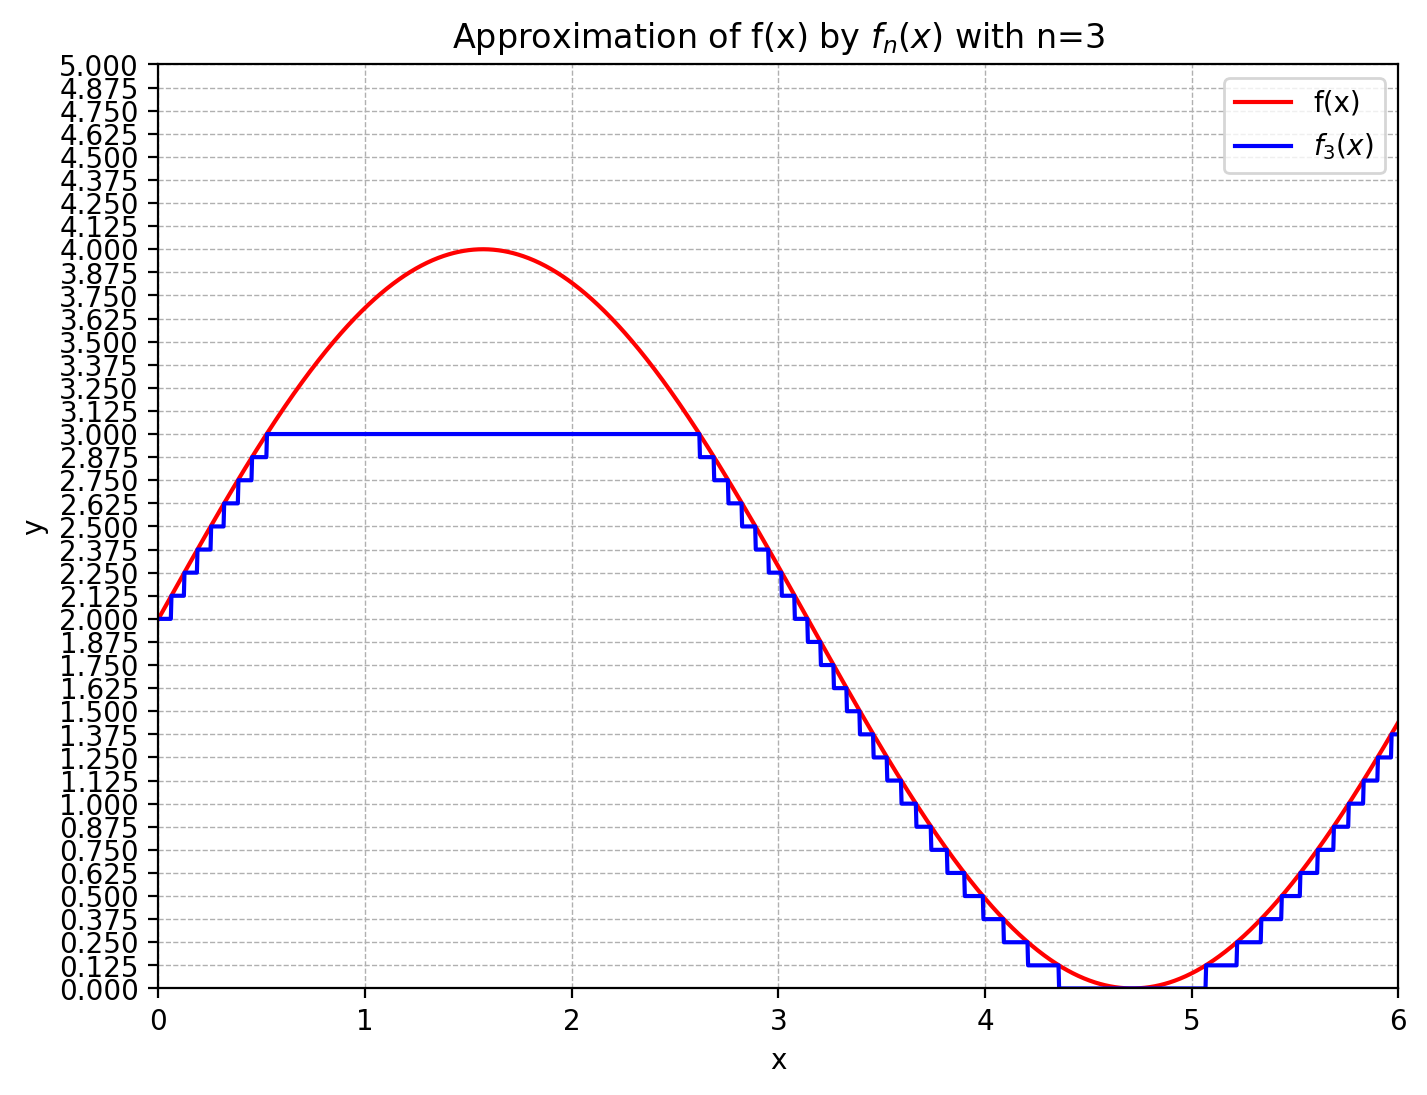
\includegraphics[width=0.6\linewidth]{fig/prop2-5.png}
        \caption{Example for Prop 2.5(1)}
        \label{fig:prop2.5}
    \end{figure}
\end{note}

\begin{note}{p.~23}
    Counting measure is simply summing up, analogously, \texttt{np.sum(x)} in numpy. 
    \begin{enumerate}
        \item $f_n(k)=f(n)\mathbf{1}_{\{n\}}(k)$, which means only when $k=n$ does $\mathbf{1}_{\{n\}}(k)=1$, thus $\sum_n f_n(k)=\sum_n f(n)\mathbf{1}_{\{n\}}(k)=f(k)$ (fix $k$ and treat $n$ as the variable). So $\sum_n f_n=f$. By Prop 2.5(3),
        \[
        \int f\mathrm{d}\mu=\int \left(\sum_{n\in\mathbb{N}}f_n\right)\mathrm{d}\mu=\sum_{n\in\mathbb{N}}\int f_n\mathrm{d}\mu
        \]
        Since $f_n$ is a simple function,
        $$
        \int f_n\mathrm{d}\mu=\int f(n)\mathbf{1}_{\{n\}}(k)\mathrm{d}\mu(k)=\sum_{k\in\mathbb{N}}f(n)\mathbf{1}_{\{n\}}(k)=f(n)
        $$
        We conclude that
        \[
        \int f\mathrm{d}\mu=\sum_{n\in\mathbb{N}}f(n).
        \]
        \item $f_n(k)=a_{n,k}$, remember that $k$ is the variable.
        \[
        \int\left(\sum_{n\in\mathbb{N}}f_n\right)\mathrm{d}\mu=
        \int\left(\sum_{n\in\mathbb{N}}a_{n,k}\right)\mathrm{d}\mu=
        \sum_{k\in\mathbb{N}}\left(\sum_{n\in\mathbb{N}}a_{n,k}\right)
        \]
        \[
        \sum_{n\in\mathbb{N}}\int f_n\mathrm{d}\mu=
        \sum_{n\in\mathbb{N}}\int a_{n,k}\mathrm{d}\mu=
        \sum_{n\in\mathbb{N}}\left(\sum_{k\in\mathbb{N}}a_{n,k}\right)
        \]
        Then use Prop 2.5(3).
    \end{enumerate}
\end{note}

\begin{note}{Cor 2.6}
    Detailed proof for equation (2.1). 
    \begin{itemize}
        \item[(Step 1)] For indicator function $f=\mathbf{1}_A$
        \[
        \int \mathbf{1}_A\mathrm{d}v=v(A)=\int \mathbf{1}_A g\mathrm{d}\mu
        \]
        by definition of integral (see Def 2.1) and $v(A)$.
        \item[(Step 2)] Extend to simple function using Prop 2.5(2),$f_n=\sum_{i=1}^n \alpha_i \mathbf{1}_{A_i}$,
        \[
        \int f_n\mathrm{d}v=\int \left(\sum_{i=1}^n \alpha_i \mathbf{1}_{A_i}\right)\mathrm{d}v=\sum_{i=1}^n\alpha_i\int \mathbf{1}_A\mathrm{d}v
        \]
        By Step 1,
        \[
        =\sum_{i=1}^n\alpha_i\int \mathbf{1}_A g\mathrm{d}\mu=\int f_n g\mathrm{d}\mu
        \]
        \item[(Step 3)] Extend to all nonnegative measurable function using Prop 2.5(1). $\exists \{f_n\}_n$ such that $f_n\uparrow f$. By Thm 2.4,
        \[
        \int f\mathrm{d}v=\lim_{n\to\infty}\uparrow \int f_n\mathrm{d}v=\lim_{n\to\infty}\uparrow \int f_n g\mathrm{d}\mu=\int f g\mathrm{d}\mu
        \]
    \end{itemize}
\end{note}

\begin{note}{Prop 2.7}
    (2) Logic: write $\infty$ as $\forall n\ge 1, \exists f(x)>n$. Call $\{f(x)>n\}$ an event, denoted by $A_n$. $\forall n\ge 1$ in set theory language is $\bigcap_{n\ge 1}$.

    Question: Does the reverse hold? Answer: No! Counterexample: $f(x)=1/x,x\in(0,1]$, and let $\mu$ be Lebesgue measure. $f<\infty$ a.e., but $\int_0^1 \frac{1}{x}\mathrm{d}x=\infty$.

    (3) To show the set such that $f(x)$ lies in $(0,+\infty)$ is measure zero, find a sequence of sets such that
    \[
    (0,+\infty)=\bigcup_{n=1}^{\infty}[1/n,+\infty)
    \]
\end{note}

\begin{note}{Prop 2.9}
    The proof appears extremely similar to Cor 2.6.
    \begin{enumerate}
        \item[(Step 1)] Let $h=\mathbf{1}_B$, then $h=1$ only when $\varphi(x)\in B, x\in \varphi^{-1}(B)$.
        \[
        \int_E \mathbf{1}_B (\varphi(x))\mu(\dif x)=\int_E \mathbf{1}_{\varphi^{-1}(B)} (x)\mu(\dif x)=\mu(\varphi^{-1}(B))=v(B)=\int_F \mathbf{1}_B(y)v(\dif y)
        \]
        \item[(Step 2)] If $h_n$ is a simple function, $h_n=\sum_{i=1}^n\alpha_i \mathbf{1}_{A_i}$.
        \[
        \int_E h_n(\varphi(x))\mu(\dif x)
        =\sum_{i=1}^n \alpha_i\int_E \mathbf{1}_{A_i}(\varphi(x))\mu(\dif x)
        =\sum_{i=1}^n\alpha_i v(A_i)
        =\int_F h_n(y)v(\dif y)
        \]
        \item[(Step 3)] For all nonnegative measurable function $h$, contruct $h_n\uparrow h$ using the method in Prop 2.5(1). By Thm 2.4 (MCT),
        \[
        \int_E h(\varphi(x))\mu(\dif x)
        =\lim_{n\to\infty}\uparrow \int_E h_n(\varphi(x))\mu(\dif x)
        =\lim_{n\to\infty}\uparrow \int_F h_n(y)v(\dif y)
        =\int_F h(y)v(\dif y)
        \]
    \end{enumerate}
\end{note}

\begin{note}{p.~34}
    ``Notice that (iii)'$\Rightarrow$(iii) thanks to the mean value theorem.''

    $\exists\xi\in(u_0,u)$ or $\in (u,u_0)$, such that
    \[
    |f(u,x)-f(u_0,x)|\le \bigg|\frac{\partial f}{\partial u}(\xi,x)\bigg|\cdot |u-u_0|\le g(x)\cdot |u-u_0|
    \]
\end{note}